\documentclass[aspectratio=169]{beamer}

\usepackage{fontspec}
\usepackage{tikz}
\usepackage{graphicx}
\usepackage{booktabs}
\usepackage{fontawesome5}
\usetikzlibrary{positioning,shapes,arrows}

% Load custom styles
\usepackage{./styles/colors}
\usepackage{./styles/theme}
\usepackage{./styles/fonts}

% Additional settings
\usetheme{Madrid}
\setbeamertemplate{navigation symbols}{}

% Presentation info
\title{YOUR PRESENTATION TITLE}
\author{Your Name}
\institute{Your Institution}
\date{\today}

\usepackage{booktabs}  % For nice tables
\usepackage{fontawesome5}  % For icons
\usepackage{tikz}  % For drawings
\usetikzlibrary{positioning,shapes,arrows}

% Custom commands for consistent styling
\newcommand{\sectionslide}[1]{%
    \begin{frame}[plain]
        \begin{center}
            \Huge\color{mainblue}#1
        \end{center}
    \end{frame}
}

\newcommand{\quoteslide}[1]{%
    \begin{frame}[plain]
        \begin{center}
            \Large\itshape
            ``#1''
        \end{center}
    \end{frame}
}

\newcommand{\bigicon}[1]{%
    \begin{tikzpicture}
        \node[minimum size=3cm,fill=lightblue,rounded corners] {\color{white}\Huge#1};
    \end{tikzpicture}
}

\begin{document}

% Title slide
\begin{frame}
\titlepage
\end{frame}

% Content slides
\begin{frame}
\frametitle{Sample Content Slide}
\begin{itemize}
    \item This is a bullet point
    \item With multiple items
    \item And more content
\end{itemize}
\end{frame}

% Two column layout example
\begin{frame}
\frametitle{Two Column Layout}
\begin{columns}[T]
    \begin{column}{0.48\textwidth}
        Left column content
    \end{column}
    \begin{column}{0.48\textwidth}
        Right column content
    \end{column}
\end{columns}
\end{frame}

% Quote slide example
\begin{frame}[plain]
\begin{center}
\large
\textit{"Your quote text here"}
\end{center}
\end{frame}


% Big concept slide with icon
\begin{frame}
\frametitle{Big concept}
\begin{columns}[T]
    \begin{column}{0.4\textwidth}
        \begin{tikzpicture}
            \fill[lightblue] (0,0) rectangle (4,4);
            \node[white] at (2,2) {\Huge \faRocket};
        \end{tikzpicture}
    \end{column}
    \begin{column}{0.6\textwidth}
        \LARGE Bring the attention of your audience over a key concept using icons or illustrations
    \end{column}
\end{columns}
\end{frame}

% Three column layout
\begin{frame}
\frametitle{In three columns}
\begin{columns}[T]
    \begin{column}{0.3\textwidth}
    \textbf{Yellow}
    \small
    Is the color of gold, butter and ripe lemons. In the spectrum of visible light, yellow is found between green and orange.
    \end{column}
    
    \begin{column}{0.3\textwidth}
    \textbf{Blue}
    \small
    Is the colour of the clear sky and the deep sea. It is located between violet and green on the optical spectrum.
    \end{column}
    
    \begin{column}{0.3\textwidth}
    \textbf{Red}
    \small
    Is the color of blood, and because of this it has historically been associated with sacrifice, danger and courage.
    \end{column}
\end{columns}
\end{frame}

% Big number slide
\begin{frame}[plain]
\begin{center}
\begin{tikzpicture}
    \node[anchor=west] at (0,0) {
        \begin{minipage}{0.8\textwidth}
            \begin{flushleft}
                {\color{yellow}\Huge \faArrowRight} {\Huge 89,526,124\$}\\[1em]
                {\large That's a lot of money}\\[2em]
                
                {\color{magenta}\Huge \faArrowRight} {\Huge 185,244} {\Huge users}\\[1em]
                {\large And a lot of users}\\[2em]
                
                {\color{lightblue}\Huge \faArrowRight} {\Huge 100\%}\\[1em]
                {\large Total success!}
            \end{flushleft}
        \end{minipage}
    };
\end{tikzpicture}
\end{center}
\end{frame}

% Process steps
\begin{frame}
\frametitle{Our process is easy}
\begin{center}
\begin{tikzpicture}[
    arrow/.style={->,thick,mainblue},
    box/.style={minimum width=3cm,minimum height=1cm}
]
    \node[box,fill=lightblue] (first) at (0,0) {First};
    \node[box,fill=mainblue,text=white] (second) at (4,0) {Second};
    \node[box,fill=magenta,text=white] (last) at (8,0) {Last};
    
    \draw[arrow] (first) -- (second);
    \draw[arrow] (second) -- (last);
    
    \node[text width=3cm,align=center,below=1cm of first] {
        \small Lorem ipsum dolor sit amet, consectetur adipiscing elit.
    };
    \node[text width=3cm,align=center,below=1cm of second] {
        \small Lorem ipsum dolor sit amet, consectetur adipiscing elit.
    };
    \node[text width=3cm,align=center,below=1cm of last] {
        \small Lorem ipsum dolor sit amet, consectetur adipiscing elit.
    };
\end{tikzpicture}
\end{center}
\end{frame}

% Device mockup slide (e.g., mobile)
\begin{frame}
\frametitle{Mobile project}
\begin{columns}[T]
    \begin{column}{0.4\textwidth}
        \textbf{Show and explain your web, app or software projects}
        \vspace{1em}
        
        Using these device mockups, you can showcase your projects in a professional way.
    \end{column}
    \begin{column}{0.6\textwidth}
        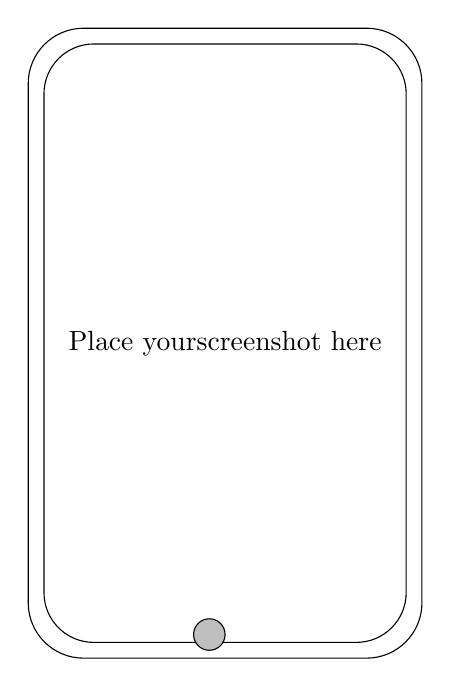
\begin{tikzpicture}
            \draw[rounded corners=20pt] (0,0) rectangle (5,8);
            \draw[rounded corners=18pt] (0.2,0.2) rectangle (4.8,7.8);
            \draw[fill=lightgray] (2.3,0.3) circle (0.2);
            \node at (2.5,4) {Place your\\screenshot here};
        \end{tikzpicture}
    \end{column}
\end{columns}
\end{frame}

% Image with caption slide
\begin{frame}
\frametitle{A picture is worth a thousand words}
\begin{columns}[T]
    \begin{column}{0.4\textwidth}
        \textbf{A complex idea can be conveyed with just a single still image}
        \vspace{1em}
        
        Making it possible to absorb large amounts of data quickly.
    \end{column}
    \begin{column}{0.6\textwidth}
        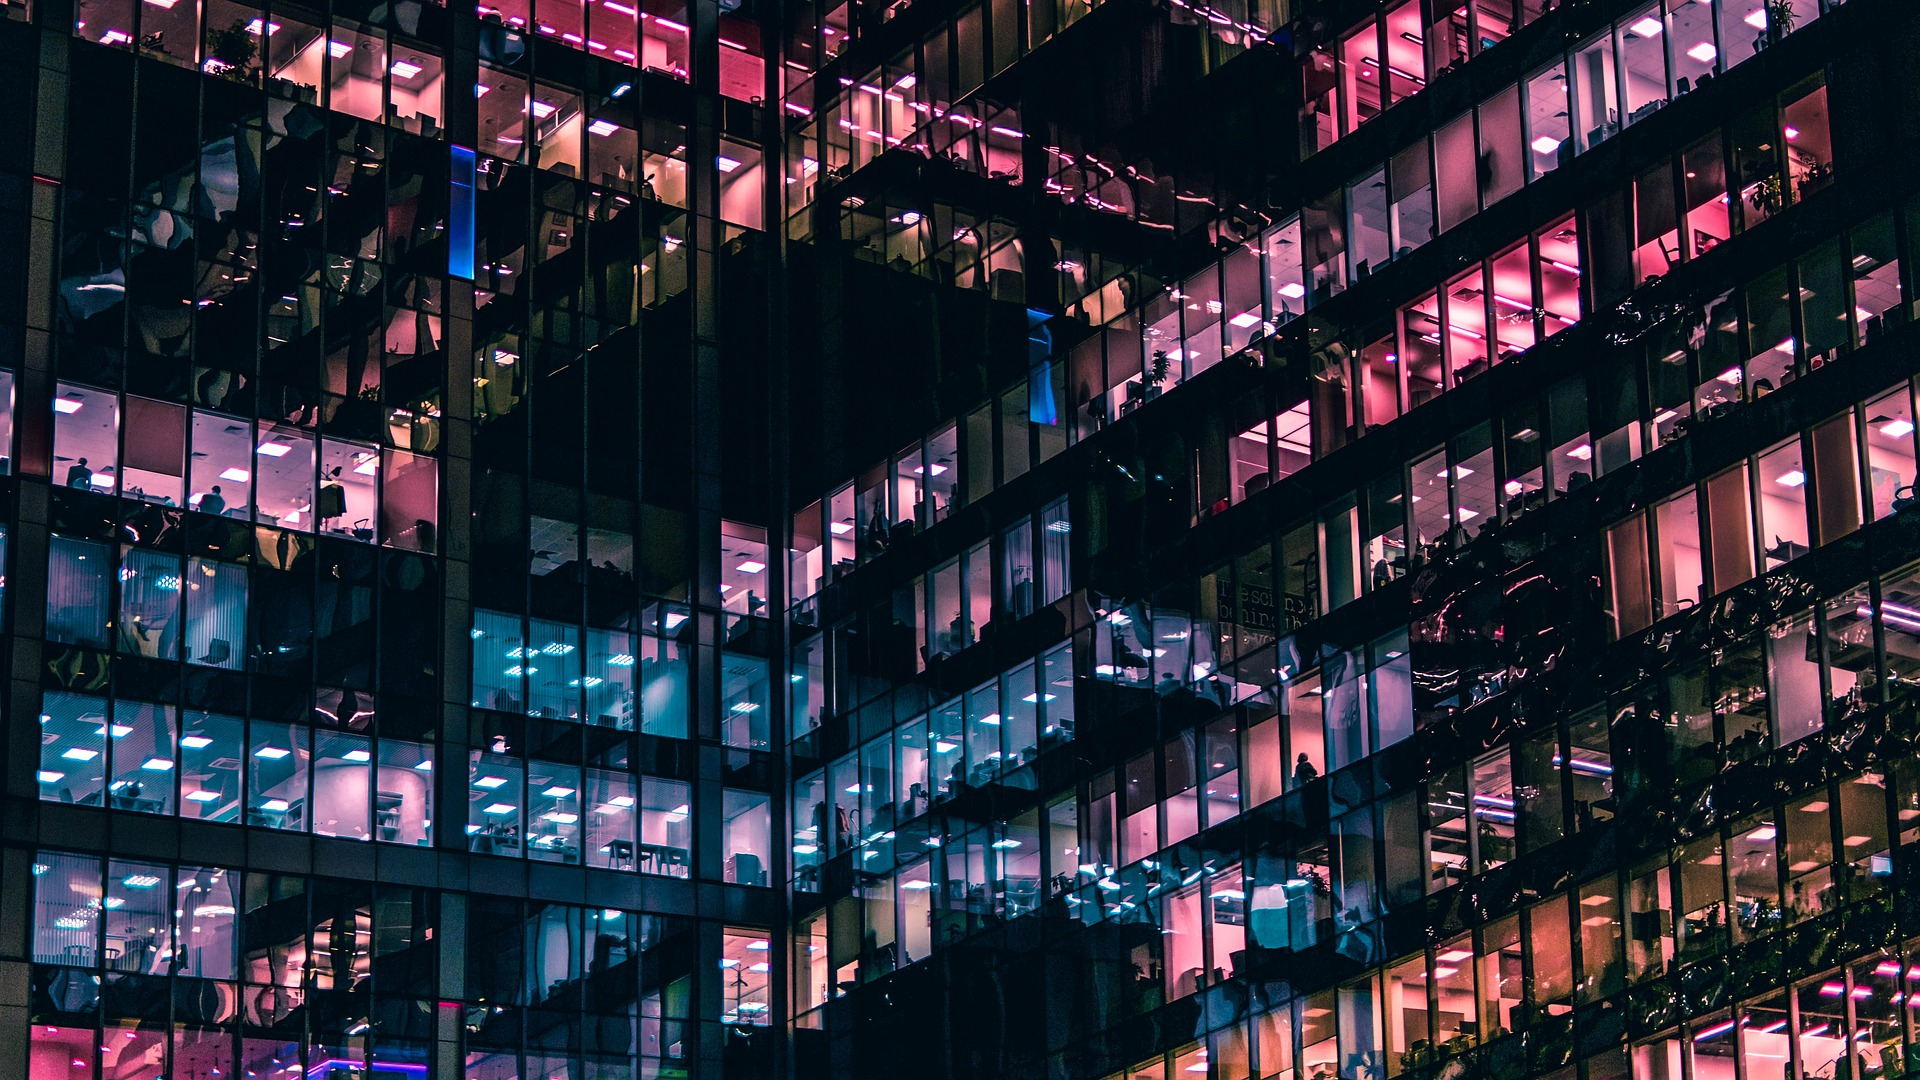
\includegraphics[width=\textwidth]{images/city.jpg}
    \end{column}
\end{columns}
\end{frame}

% Table slide
\begin{frame}
\frametitle{And tables to compare data}
\begin{center}
\begin{tabular}{lccc}
\toprule
& A & B & C \\
\midrule
Yellow & 10 & 20 & 7 \\
Blue & 30 & 15 & 10 \\
Orange & 5 & 24 & 16 \\
\bottomrule
\end{tabular}
\end{center}
\end{frame}

% Icon grid slide
\begin{frame}
\frametitle{Available icons}
\begin{center}
\begin{tikzpicture}[icon/.style={minimum size=1cm}]
    \foreach \i in {0,...,4} {
        \foreach \j in {0,...,4} {
            \node[icon] at (\i*1.2, -\j*1.2) {\faIcon};
        }
    }
\end{tikzpicture}
\end{center}
\end{frame}



% Closing slide
\begin{frame}
\begin{center}
\Huge Thanks!\\[1em]
\large Any questions?\\[1em]
\normalsize
Contact: your@email.com
\end{center}
\end{frame}

\end{document}